\documentclass[11pt,a4paper]{article}
\usepackage{fullpage}
\usepackage{amsmath}
\usepackage{amssymb}
\usepackage{amsfonts}
\usepackage{mathtools}
\usepackage{titlesec}
\usepackage{graphicx}
\usepackage{float}
\usepackage{wrapfig}
\usepackage{multicol}
\usepackage{caption}
\usepackage{hyperref}
\usepackage{apacite}
\usepackage{tabularx}
\usepackage{multirow}
\usepackage{subcaption}
\usepackage[noend]{algpseudocode}
\usepackage[nothing]{algorithm}
\usepackage{array}
\newcolumntype{T}{>{\tiny}l} % define a new column type for \tiny
\newcolumntype{H}{>{\Huge}l} % define a new column type for \Huge
\newcolumntype{P}[1]{>{\centering\arraybackslash}p{#1}}

\usepackage{stackengine}
\newsavebox\mybox
\newcommand\Includegraphics[2][]{\sbox{\mybox}{%
\includegraphics[#1]{#2}}\abovebaseline[-.5\ht\mybox]{%
\addstackgap{\usebox{\mybox}}}}

\algnewcommand\And{\textbf{and} }
\algnewcommand\Or{\textbf{or} }

\def\SPSB#1#2{\rlap{\textsuperscript{{#1}}}\SB{#2}}
\def\SP#1{\textsuperscript{{#1}}}
\def\SB#1{\textsubscript{{#1}}}


\DeclarePairedDelimiter{\ceil}{\lceil}{\rceil}
\DeclarePairedDelimiter\floor{\lfloor}{\rfloor}
\newcommand*{\field}[1]{\mathbb{#1}}%

\begin{document}
%\title{\textbf{Rendering Master Project \\
%WS 2021/2022 \\
%Implementing and Analysing Acceleration Data Structures in Ray tracing}}
%\author{Report by Adil Rabbani \\ Supervised by: Prof. Dr.-Ing. Matthias Teschner}
%\date{4.11.2021}
%\maketitle

\begin{titlepage}

	\begin{center}
	Chair of Computer Graphics - Albert-Ludwigs-University of Freiburg \\
	\line(1, 0){300}\\
	[0.25in]
	\huge{Rendering Master Project \\
					   WS 2021/2022} \\
	\line(1, 0){300}\\
	[0.75in]
	\textsc{\LARGE Implementation and Analysis of Acceleration Structures in Ray tracing}\\
	
	\begin{figure}[H]
		\centering
		\captionsetup{justification=centering,margin=2cm}
		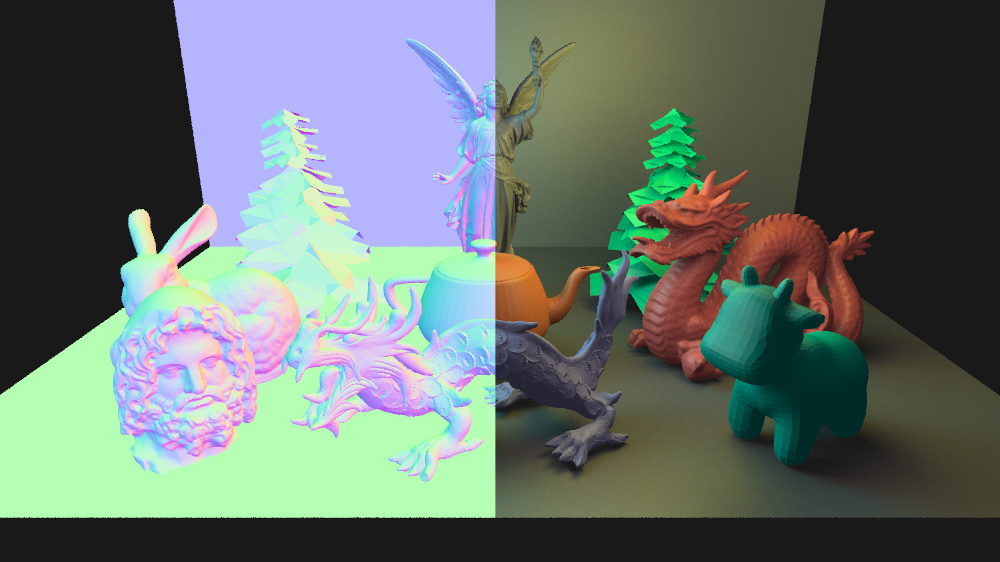
\includegraphics[width=0.8\textwidth]{cover_image}
	\end{figure}
	
	\textsc{\Large Report by Adil Rabbani \\ Supervised by Prof. Dr.-Ing. Matthias Teschner\\}
	\textsc{\large Submitted on: 03.10.2022}

	\end{center}

\end{titlepage}

\noindent
\textbf{\Large{Acknowledgments}}
\\~\\
This project and report is not the work of the author alone. The author thanks his supervisor \textbf{Prof.
	Dr.-Ing. Matthias Teschner} for the discussions and constant support throughout this project. Moreover, all the papers and resources used have been a great help in understanding as well as explaining each concept used in this project. All resources as well as illustrations have been referenced wherever necessary. Illustrations which are not referenced were drawn by the author himself.
\\~\\
\noindent
\textbf{\Large{About the cover}}
\\~\\
The cover image was rendered using a ray tracer implemented in a previous semester. Peter Shirley's Ray Tracing in One Weekend \cite{Shirley2020RTW1} and Kevin Suffern's Ray Tracing from the Ground up \cite{suffern2016ray} were an important resource in implementing most of the functionalities in that ray tracer. The same ray tracer would be used throughout this report. The image was rendered first using normal mode, which colors each point according to the normal at that point and then rendered again, using Phong Illumination and area lights spread out in between the scene. The images were then cropped half and merged using a photo editor. The image would have been impossible to render in a reasonable time without the acceleration structures discussed in this report. The scene will be discussed in more detail, later in the report. Special thanks to McGuire Computer Graphics Archive \cite{McGuire2017Data} for providing 3D models for Stanford Dragon \cite{stanforddragon}, Serapis Bust \cite{serapis}, Scrub Pine Tree \cite{pinetree} and Utah teapot \cite{utahteapot}. Also thanks to Alec Jacobson's common 3d test models repository \cite{common3dmodels} for the Stanford XYZ Dragon \cite{stanfordxyzdragon}, Stanford Lucy \cite{stanfordlucy}, Stanford Bunny \cite{stanfordbunny} and Caltech Spot \cite{spot}.

\pagebreak
\tableofcontents
\pagebreak

\section{Abstract}
Acceleration data structures play an important role in any ray tracer, reducing the amount of intersections of each ray with objects in our scene. Mainly, there are two broad categories of acceleration structures namely, \textbf{spatial subdivision} and \textbf{object subdivision}. Spatial subdivision algorithms divide 3D space into regions and record which primitives overlap which regions. On the other hand, object subdivision algorithms progressively break the objects in the scene into smaller sets of objects. This report implements and investigates two different kinds of acceleration data structures namely, \textbf{Bounding Volume Hierarchies (BVH)} and \textbf{Uniform Grid}. BVH is an example of object subdivision acceleration structure while Uniform Grid is an example of spatial subdivision. The report would further analyze in what scenarios these structures are preferred from one another and what are the pros and cons of using either of them.
\\~\\
\noindent
\textbf{Keywords:} [ray tracing] [acceleration structure] [grid] [hierarchies] [object subdivision] [spatial subdivision]

\section{An overview of Ray tracing}
\textbf{Ray tracing} is a method to generate photo-realistic images which resemble closely to how we perceive things in real life. This is due to the fact that it tries to simulate light traveling in a virtual scene by using principles from \textbf{geometric optics} \cite{geometricoptics}. Geometric optics is a model of optics that describes light propagation in terms of rays and that these rays travel in straight lines.  We start by casting rays from each of the pixel of our
screen from the view position. As we do this, we hit various objects in our scene. This is evaluated by
ray-primitive intersection tests. As an object is hit, we compute illumination at that point depending
on how far the position is from a light source. As we also want to create shadows in our scene, when
a point in our scene is hit by a ray, we shoot another ray from that position, towards
the light source. If this ray hits another object on its way towards the light source, we conclude that
the point we are shading is in a shadow. In ray tracing, if one object is in front of another object, we
shade the object which is closest from the ray origin. This process of sending rays through each pixel,
evaluating ray-primitive intersection tests, and computing illumination at each point in our scene makes
ray tracing very performance intensive.

\begin{figure}[H]
	\centering
	\captionsetup{justification=centering,margin=2cm}
	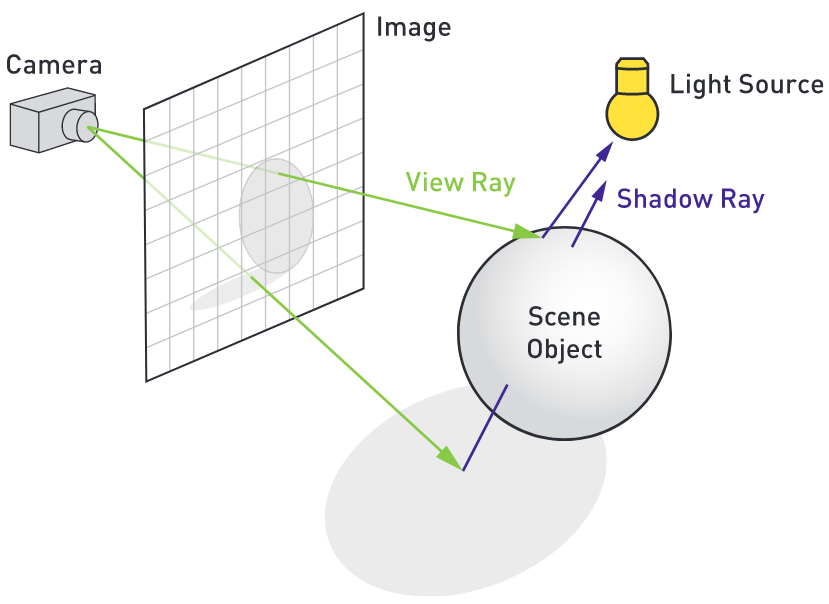
\includegraphics[width=0.45\textwidth]{raytracing_gems}
	\caption{Visualization of how ray tracing works. \protect\cite{haines2019ray}}
\end{figure}
\noindent
But what makes ray tracing appealing
is the fact that this process of rendering images allows to create highly realistic images because it can accurately
model light traveling in our scene. It might seem very difficult to differentiate the rendered image below from a real life photo.

\begin{figure}[H]
	\centering
	\captionsetup{justification=centering,margin=2cm}
	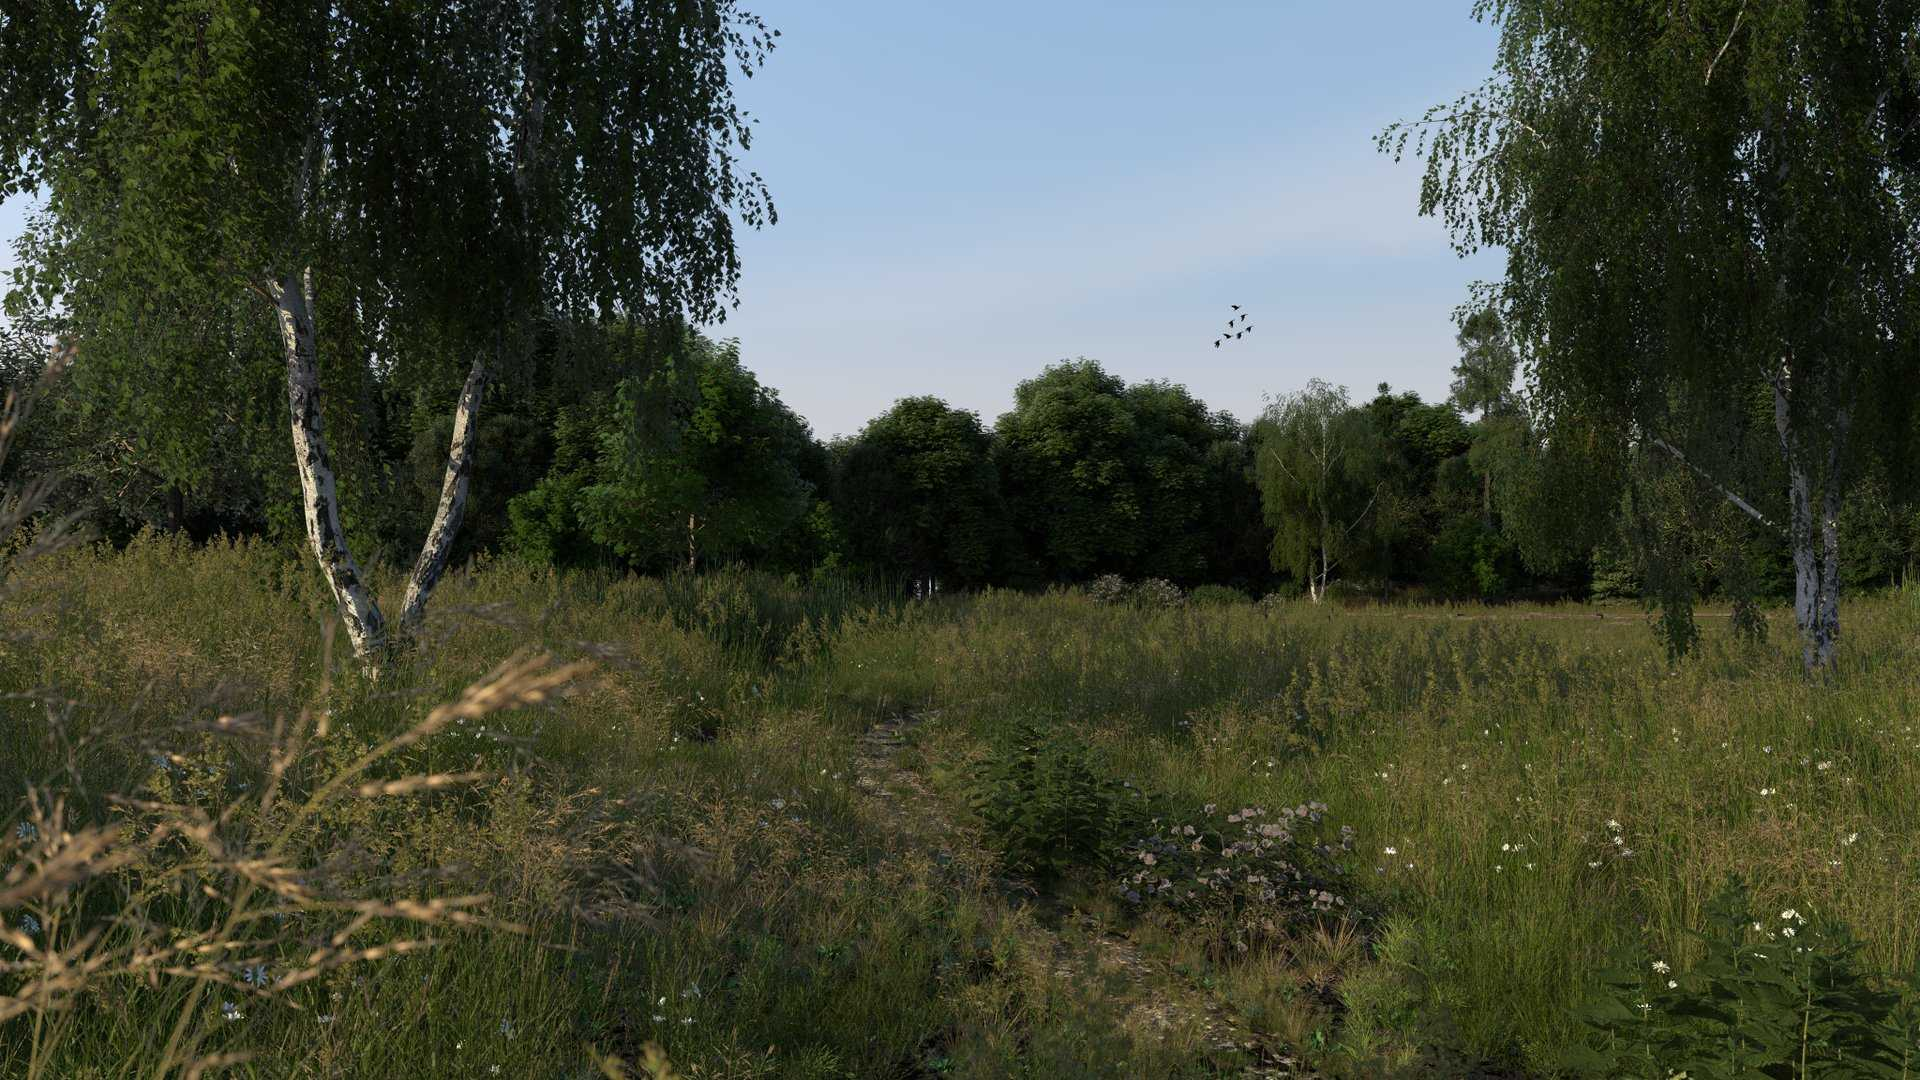
\includegraphics[width=0.4\textwidth]{landing}
	\caption{A nature scene from pbrt rendered using ray tracing. \protect\cite{pharr2016physically}}
\end{figure}

\noindent
For this reason, ray tracing is often used for \textbf{offline rendering}. We first create an image or a series of images (frames), exporting them to a specific image format. And then, these series of frames can be viewed later. This is often used for computer generated movies as well as advertisements. In fact, Disney's renderer \textbf{Hyperion} is a physically based path tracer (one of the commonly used methods in ray tracing). 

\begin{figure}[H]
	\centering
	\captionsetup{justification=centering}
	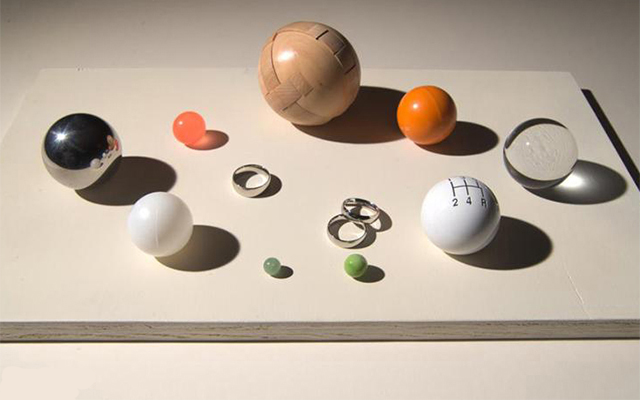
\includegraphics[width=.35\textwidth]{real_photo}\quad
	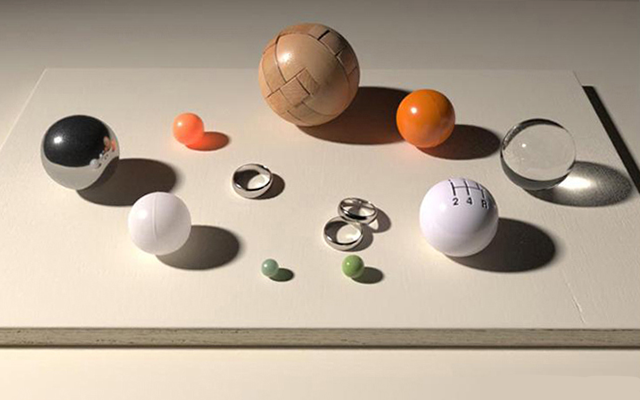
\includegraphics[width=.35\textwidth]{hyperion}\quad
	\caption{A comparison of a real photo (left) and an image rendered using hyperion (right). \protect\cite{burley2018design}}
\end{figure}

\section{Importance of acceleration structures}
Considering that many complex scenes can contain millions or even billions of primitives (triangles in most cases); it is impossible to render such complex scenes in a reasonable time, without using any acceleration structure. Tracing even a single ray with our naive brute force approach would result in a time complexity of ($O(N.M)$) where $N$ is the number of pixels in our image and $M$ is the number of primitives in our scene; as the ray needs to be tested against each primitive in the scene to find the closest intersection. 
\\~\\
\noindent
As more and more features are added to the ray tracer, the number of rays sent from the view point towards the scene also increases. One example of a very common method for smoothing out the rendered image is anti-aliasing. In order to do anti-aliasing, we need to send more than one ray per pixel and average the color received for each ray. This means that doing 5x anti-aliasing will result in a smoother image but this would also increase the number of rays sent per pixel by $5$. 
\\~\\
\noindent
If we implement different materials that model reflections; the rays sent towards the scene are then reflected from these materials and then tested again with other objects in the scene as they are reflected. Shadow rays as previously discussed, also require us to send a ray towards a light when a primary ray hits a surface. This means that for each ray hit, we send an additional ray towards the light source to compute shadows. Area lights are one example of a light source which simulates soft shadows and these lights are composed of a region of light instead of just one point in space. One way to achieve area light effects is to arrange point lights in a particular region in a grid. This means that now we need a grid of 3x3 or a 5x5 point lights, thereby also increasing the number of shadow rays sent for each of those lights. Moreover, moving on towards more advanced ray tracing techniques such as Monte Carlo Ray tracing requires us to send hundreds of rays per pixel in order to reduce noise in our images.
\\~\\
\noindent
All these examples demonstrate that the number of rays sent towards the scene, keeps on increasing as more and more features are added to the ray tracer. A ray sent towards a particular region of the scene should only intersect with primitives in that region while ignoring majority of the primitives in the scene and hence testing all primitives in a scene for each ray is extremely wasteful for time as well as space. Since we are only interested for the closest intersection of a ray with a primitive, there are acceleration structures which help in grouping as well as ordering many primitives in the scene and check if a ray hits any of them. This speeds up the rendering process as many of the ray-object intersection tests are too expensive to compute and reducing these intersection tests can greatly reduce the amount of time and space required for rendering the image. And so, this is a clear motivation for acceleration structures in ray tracing. We will begin our discussion of acceleration structures with a spatial subdivision technique known as \textbf{Uniform Grid}.

\section{Uniform Grid}
\subsection{Concept}
Spatial subdivision or space subdivision is a technique to reduce intersections with the primitives in the scene by partitioning the space of the scene into regions or cells. Once the space is subdivided into cells, each cell has their own list of objects. This helps reducing the number of intersection tests because when a ray is traced in a particular region, we can ignore the objects that are not in the same region as the ray intersects. A very simple example is shown in the figure below:
\begin{figure}[H]
	\centering
	\captionsetup{justification=centering,margin=2cm}
	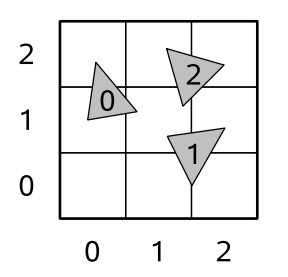
\includegraphics[width=0.18\textwidth]{uniformgrids}
	\caption{A grid with three triangles overlapping the cells. \protect\cite{lagae2008compact}}
\end{figure}
Figure.4 shows a 3x3 grid used to partition a scene consisting of 3 triangles. It is obvious that when our ray intersects cell $(1, 0)$, we can just test the objects that are contained in that cell (triangle 0) and we need not care about the triangles in other regions. This way of partitioning space into cells or voxels (in 3D) is called a \textbf{uniform grid}.
Uniform grid was one of the first proposed acceleration structures \cite{fujimoto1986arts} in rendering. As discussed previously, the idea is to divide the 3D space into a 3D grid. The approach is good as it automatically divides the objects into smaller parts which are faster to test than testing an entire 3D model consisting of millions of triangles.
\subsection{Implementation}
The uniform grid implementation that is used in this project is from the paper \textbf{Compact, Fast and Robust Grids for Ray Tracing}\cite{lagae2008compact}. The paper presents a compact grid method which consists of a static data structure for representing a grid with minimal memory requirements, more specifically exactly one index per grid cell and exactly one index per object reference. This means that we will only be storing just one index for a cell in our grid and only one index to reference an object in our scene. All acceleration data structures consist of two phases, i.e \textbf{constructing} the structure and \textbf{traversing} it. We will divide our discussion in the same way.
\subsubsection{Construction}
A uniform grid structure first require us to calculate the number of cells in our grid or more accurately the resolution of the grid denoted by $M$. The number of cells should be linear in the number of objects $N$ in our scene \cite{devillers1988methodes}:
\begin{equation}
M = \rho N,
\end{equation}
where $\rho$ is called the grid density which is a scalar value. The number of cells $M$ is equal to the product of the resolution of the grid in each dimension. The resolution of the grid $M_{x} \times M_{y} \times M_{z}$ is therefore given by:

\begin{equation}
M_{i} = S_{i} \sqrt[3]{\frac{\rho N}{V}}\;\;\;\; (i \in \{x,\;y,\;z\})
\end{equation}
where $S_{i}$ is the size of the bounding box of the grid in dimension $i$ i.e $(max_{i} - min_{i})$ and $V$ is the volume of the bounding box i.e $(S_{x} * S_{y} * S_{z})$.  The value of $\rho$ in the above formula is debatable and often chosen between $5$ to $10$. Different papers suggest different values but the paper \cite{lagae2008compact} suggests to use a value of $4$ which is based on the \textbf{time to image} rather than the render time as shown below:
\begin{figure}[H]
	\centering
	\captionsetup{justification=centering,margin=2cm}
	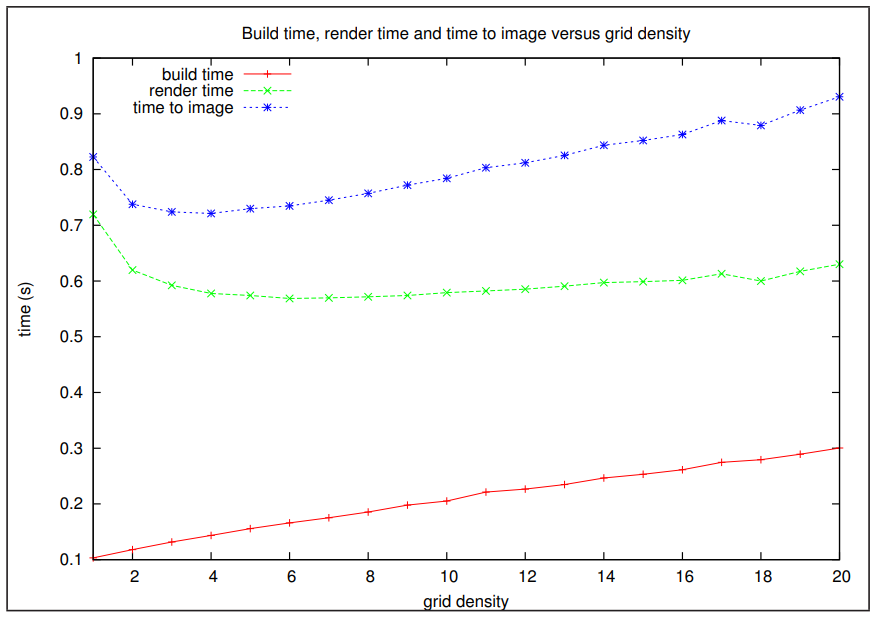
\includegraphics[width=0.55\textwidth]{grid_density_graph}
	\caption{Grid density. Build time (red), render time (green) and
time to image (blue) versus grid density for the Happy Buddha
scene. A grid density of 4 minimizes the time to image. \protect\cite{lagae2008compact}}
\end{figure}
It can be seen that the value $4$ gives a nice balance for the time it takes to build the structure and the time it takes to render the image.
\\
\noindent

The next question we need to answer when building a uniform grid is how to insert objects in our cells. One way to do it is to use axis aligned bounding box (AABB) for each primitive in our scene and then test it if it overlaps with the cell in our grid. This is fast, however, some primitives end up in cells that overlap the bounding box but not the primitive itself which results in longer render times. More complex primitive cell tests exist but then they are slower to test. We therefore, use the bounding box method to insert primitives in our cell.
\\
\noindent

In order to get an intuition of how the structure is built, we will briefly discuss two other simpler methods of building uniform grids. One traditional way to represent grids with object references is by using linked lists. This is illustrated in figure 6. Figure 6(a) shows a simple scene with three triangles which is subdivided into cells of a 2D grid. A linearized 1D version of the same grid is also shown. Here, it can be seen that a cell index $(1, 0)$ in 2D is the same cell with the index (3) in 1D.
\begin{figure}[H]
	\centering
	\captionsetup{justification=centering}
	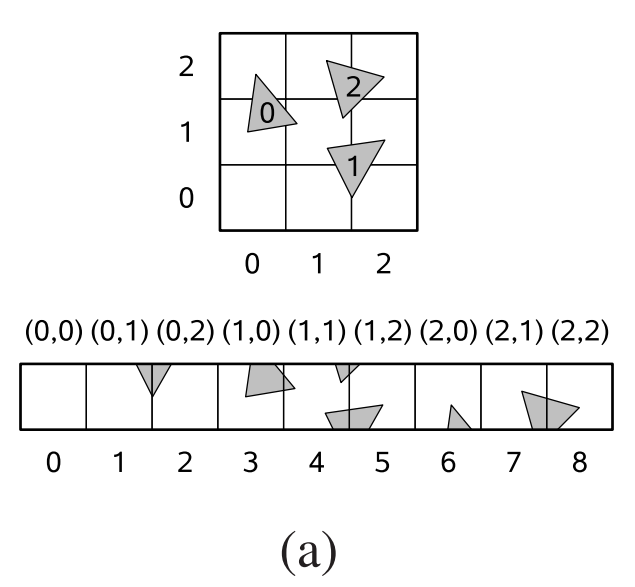
\includegraphics[width=.28\textwidth]{uniformgrids1}\quad
	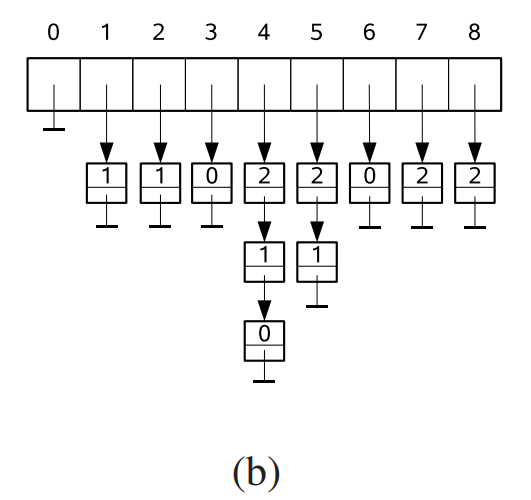
\includegraphics[width=.28\textwidth]{uniformgrids2}\quad
	\caption{a) A grid with three triangles overlapping the cells and the linearized 1D version of the grid. b) A traditional grid data structure using linked lists. \protect\cite{lagae2008compact}}
\end{figure}
Figure 6(b) shows how the references are stored in each index of the linearized array. Each cell index points to a linked list which is empty if there are no primitives in that cell and contains nodes if a cell contains primitives. It can be seen that the cell index (1, 1) which is cell index (4) in the linearized array contains a linked list of 3 objects which are three triangles overlapping the cell in the scene. Another method to build the uniform grid structure is to use dynamic arrays. This is illustrated in figure 7(c).
\begin{figure}[H]
	\centering
	\captionsetup{justification=centering}
	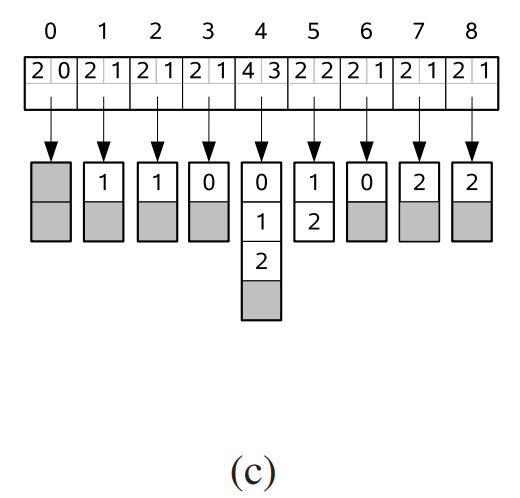
\includegraphics[width=.3\textwidth]{uniformgrids3}\quad
	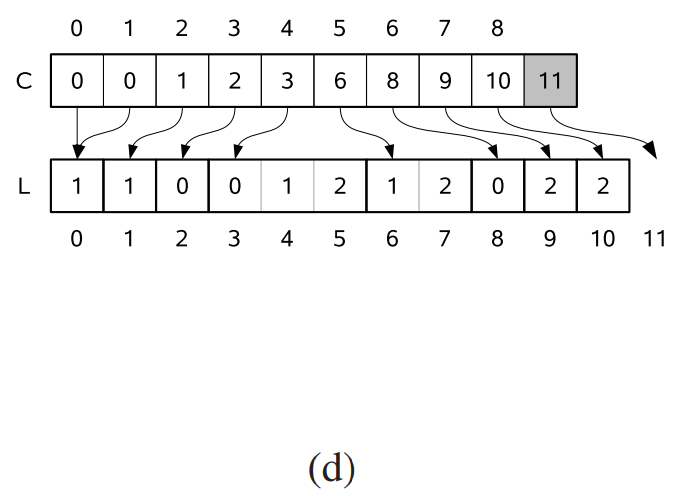
\includegraphics[width=.3\textwidth]{uniformgrids4}\quad
	\caption{c) A traditional grid data structure using dynamic arrays. d) The compact grid data structure implemented in this project.
 \protect\cite{lagae2008compact}}
\end{figure}
The first array again represents the linearized cells in our grid, while each index of the array also maintains an array with a size depending on the number of objects in a specific cell. When the size is about to exceed the capacity, a new array with a larger capacity is allocated and the old array is copied and freed. We can observe that the array index 4 which represents cell (1, 1) in our grid contains an array with a size larger than other indexes hence the name, dynamic arrays.

\noindent
\\
Both the implementations described so far have a large memory overhead as they support insertion as well as removal of objects. However, if a grid is rebuilt from scratch every frame, dynamic structures like these are not needed. We now move towards the implementation described in the paper. This is illustrated in figure 7(d). The compact grid structure has two static arrays. The array $L$ consist of the concatenation of all object lists i.e all the objects overlapped by cells are concatenated in this array. The array $C$ stores for each cell, the offset of the corresponding object list in $L$ i.e array $C$ tells us where to index array $L$ in order to fetch objects overlapped by that cell in $C$.

\noindent
\\
Array $L$ is a 1D array while array $C$ is a 3D array of size $M_{x} \times M_{y} \times M_{z}$ which is linearized in row major order into a 1D array of size M. The array $C$ can be indexed by:
\begin{equation}
C[z][y][x] = C[(((M_{y} * z) + y) * M_{x}) + x]
\end{equation}
The number of objects contained in a specific cell can be given by $C[i+1] - C[i]$. This does not hold true for the last object list and so we extend array $C$ by one position.
\\
\noindent

Now we'll discuss how to build the compact grid. First, the scene bounding box is computed. This is done by simply going through all objects in our scene and merging their bounding boxes. Once, we have the scene bounding box, we can compute $S_{i}$ (size of the scene bounding box in dimension $i$) where $i \in {x, y, z}$, the $V$ (volume of the scene bounding box) and by using equation $(2)$ with $\rho = 4$, get the resolution of the grid $M$. Here $M$ is the resolution of the grid in all 3 dimensions or $M_{x} \times M_{y} \times M_{z}$. Once, we have $M$, we can allocate array $C$ which is of the same size and initialize all its entries to 0. We also compute the cell dimension which is constant for all cells and given by:

\begin{equation}
D_{i} = \frac{S_{i}}{M_{i}}\;\;\;\; (i \in \{x,\;y,\;z\})
\end{equation}

Next, we go through all primitives in our scene, computing their bounding box one by one, converting them to cell coordinates and checking if a primitive overlaps a cell or more than one cell. This is done by subtracting the minimum of the scene bounding box from the minimum of the bounding box of the primitive and dividing it by cell dimension $\boldsymbol{D}$, to get the first cell that overlaps that primitive. The same process is done again but this time, subtracting the minimum of the scene bounding box from the maximum of the bounding box of the primitive and dividing it by cell dimension to get the last cell that overlaps that primitive. Note that both these values need to be clamped between $0$ (the first cell) and the grid resolution (the last cell) in our grid.
\begin{equation}
	\boldsymbol{first_{cell}} = \lfloor \frac{\boldsymbol{primitive_{AABB_{min}}} - \boldsymbol{scene_{AABB_{min}}}}{\boldsymbol{D}} \rfloor
\end{equation} 
\begin{equation}
	\boldsymbol{last_{cell}} = \lfloor \frac{\boldsymbol{primitive_{AABB_{max}}} - \boldsymbol{scene_{AABB_{min}}}}{\boldsymbol{D}} \rfloor
\end{equation} 
\noindent
Now we iterate from the first cell to the last cell to get all cells overlapped by the primitive. By computing the linearized index using equation $(3)$ we increment the index in cell array $C$ for all overlaps.
\\
\noindent
\\
There is a nice trick in the algorithm. Rather than computing for each cell the offset to its object list, the offset to the next object list is computed. That is, $C[i]$ records the offset of the object list of the cell with 1D index $i+1$. In simpler words, $C[i]$ points to one past the end of the object list of the cell with 1D index $i$. This is done by:
\begin{equation}
C[i] = C[i] + C[i-1]\;\;\;\;(where\;\;i\;=\;0\;\;to\;\;M)
\end{equation}
\\
\noindent
The joint size of the object list is then given by $C[M - 1]$. And that is the value that is used to allocate array $L$. Primitive indices are now inserted in array $L$ by reversely iterating over all primitives, and for each cell overlapped by the primitive, decrementing the offset of the cell and storing the primitive index at that offset. This is done by:
\begin{equation}
L[--C[j]] = i\;\;\;\;(where\;\;i\;=\;N-1\;\;to\;\;0)\;\;for\;\;each\;\;cell\;\;j\;\;overlapped\;\;by\;\;primitive\;\;i
\end{equation}
After this operation the cell array $C$ contains the correct offsets, since each offset was decremented the appropriate number of times.
\subsubsection{Illustrated example}
The construction of arrays $C$ and $L$ is illustrated using a simple example below:
\begin{figure}[H]
	\centering
	\captionsetup{justification=centering}
	\includegraphics[width=.4\textwidth]{compact_grid_1}\quad
	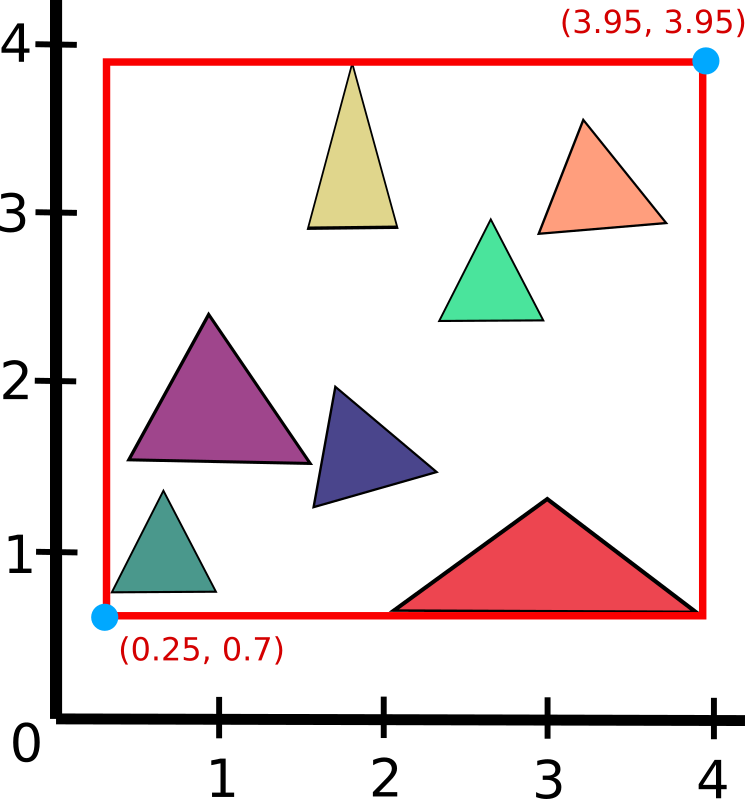
\includegraphics[width=.4\textwidth]{compact_grid_2}\quad
	\caption{A scene with 7 triangles with its bounding box calculated.}
\end{figure}
\noindent
The scene bounding box has a minimum at $(0.25, 0.7)$ and the maximum at $(3.95, 3.9)$. For simplicity of calculations we will keep maximum at $(4, 4)$. The size of the bounding box $(S_{x}, S_{y})$ is then calculated as $(max - min)$ with a value, $(3.75, 3.3)$. And the volume is calculated as $S_{x} * S_{y}$ giving a value $12.375 \approx 12.4$. We can then calculate the resolution of the grid using equation (2) above. And keeping density $\rho=4$, we get $(M_{x}, M_{y})$ as:
\begin{equation}
	M_{x}=3.75 \sqrt[3]{\frac{4(7)}{12.4}}=4.919 \approx 5
\end{equation} 
\begin{equation}
M_{y}=3.3 \sqrt[3]{\frac{4(7)}{12.4}}=4.329 \approx 4
\end{equation} 
So the grid resolution is $5 \times 4$. We get the cell dimension $(D_{x}, D_{y})$ from equation (4) above, giving $(0.75, 0.825)$. This cell dimension can then be used to subdivide the space equally into cells as:
\begin{figure}[H]
	\centering
	\captionsetup{justification=centering}
	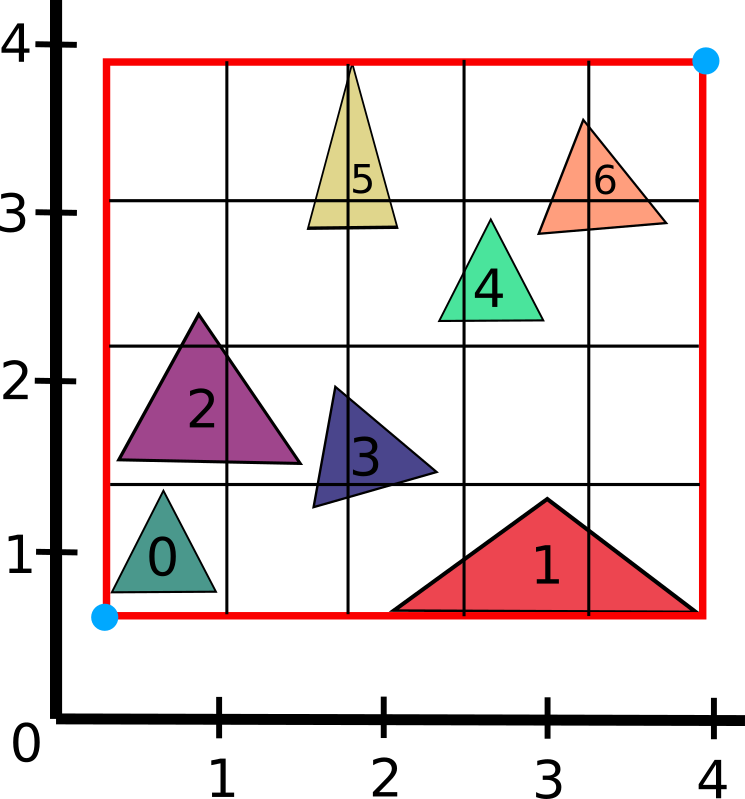
\includegraphics[width=.3\textwidth]{compact_grid_3}\quad
	\caption{Scene subdivided into cells.}
\end{figure}
\noindent
\begin{figure}[H]
	\centering
	\captionsetup{justification=centering}
	
\includegraphics[width=.65\textwidth]{compact_grid_4}\quad
	\caption{Array $C$ initialization. Size is $5 * 4 = 20$.}
\end{figure}
\noindent
\begin{figure}[H]
	\centering
	\captionsetup{justification=centering}
	
\includegraphics[width=.65\textwidth]{compact_grid_5}\quad
	\caption{Array $C$ after 1st iteration. Counting primitive overlaps in each cell.}
\end{figure}
\begin{figure}[H]
	\centering
	\captionsetup{justification=centering}
	
\includegraphics[width=.65\textwidth]{compact_grid_6}\quad
	\caption{Array $C$ after 2nd iteration. Accumulation and expansion of one index as mentioned in (3) and (7) above.}
\end{figure}
\begin{figure}[H]
	\centering
	\captionsetup{justification=centering}
	
\includegraphics[width=.65\textwidth]{compact_grid_7}\quad
	\caption{Array $L$ initialization. Size equal to value in last index of $C$.}
\end{figure}
\begin{figure}[H]
	\centering
	\captionsetup{justification=centering}
	
\includegraphics[width=.7\textwidth]{compact_grid_8}\quad
	\caption{Array $C$ and $L$. Reverse iteration over primitives as mentioned in (8) above.}
\end{figure}
\noindent
Let's check cell $13$, the one that overlaps triangles $4$ and $6$. We check if the value in cell $13$ is less than the value in the cell after that, and it is true $(14 < 16)$. We then fetch the value in the $C$ array at index $13$ which gives us $14$. Now we arrive at index $14$ in array $L$ which gives us the triangle $4$ that overlaps that cell. We check if the value in the next cell ($14$) in array $C$ is less than the value in the cell ($15$) after that, and it is true ($16 < 17$). So we fetch the value in $C$ array at index $14$ which gives us $16$. Now we arrive at index $16$ in array $L$ giving us the other triangle $6$ that overlaps that cell. Our check if the current cell value is less than value in the next cell fails this time ($17 < 17 = false$) so we exit.
\subsubsection{Traversal}

The  traversal algorithm for 3D grid presented in this report is an implementation of the paper \textbf{A Fast Voxel Traversal Algorithm for Ray Tracing}\cite{amanatides1987fast}. The very first step in our algorithm is to check if the ray even enters the bounds of our scene. This is done by checking if the ray intersects the bounding box of the scene at all, which is also the place where our bounds of the grid start. If there is no intersection, we return without doing any computation. However, if the ray does intersect the scene bounding box, we have to go through a two step process: initialization of the variables and incremental traversal of the grid. 

\begin{enumerate}
\item \textbf{Initialization}
\\ The initialization phase starts with identifying which voxel the ray intersects with at first. This is the voxel which we will use to incrementally go through the grid. In order to know which voxel our ray starts in, we first need to know where does the ray actually start from and where does it end. To get $\boldsymbol{r_{start}}$ and $\boldsymbol{r_{end}}$:
\begin{equation}
\boldsymbol{r_{start}} = \boldsymbol{r_{o}} + \boldsymbol{r_{dir}} * t_{min}
\end{equation}
\begin{equation}
\boldsymbol{r_{end}} = \boldsymbol{r_{o}} + \boldsymbol{r_{dir}} * t_{max}
\end{equation}
$\boldsymbol{r_{o}}$ and $\boldsymbol{r_{dir}}$ being the ray origin and ray direction. $t_{min}$ and $t_{max}$ are the scalar $t$ values which indicate from where do we need to start and end checking for objects in our scene or also known as the visibility area. These are typically set to $0.001$ and $infinity$ (or a large value) respectively. When we have both $\boldsymbol{r_{start}}$ and $\boldsymbol{r_{end}}$ we can get the first voxel that intersects with our ray by:
 \begin{equation}
i_{start} = \lfloor \frac{(r_{start_{i}} - scene_{AABB_{min_{i}}})}{D_{i}} \rfloor \;\;\;\; (i \in \{X,\;Y,\;Z\})
\end{equation}
\\
We calculate $i_{start}$ above for each $x$, $y$ and $z$ coordinate of our voxel respectively and then we can easily use equation (3) above to get the voxel from linearized array $C$. The above equation (13) needs to be clamped in between $0$ and grid resolutions $M_{x} - 1$, $M_{y} - 1$ and $M_{z} - 1$ respectively, so we always get a value which is inside our grid. Once we have $X_{start}$, $Y_{start}$ and $Z_{start}$, we need to compute $X_{end}$, $Y_{end}$ and $Z_{end}$ as well by using $\boldsymbol{r_{end}}$ in place of $\boldsymbol{{r_{start}}}$ in equation (13). After this, we need 3 more variables for each coordinate after which we can start the traversal. The 3 variables are the $step$, $tDelta$ and $tMax$ values:
\begin{enumerate}
\item \textbf{step}: This is the value which decides if the step in our traversal is positive, negative or zero. Or in other words, for stepX, are we going from left to right (positive), right to left (negative) or we don't want to change this coordinate at all (zero) in our traversal of voxels. It must be obvious that this is just the slope or the direction of our ray and we can set this value by checking if $r_{dir_{x}}$ is positive, negative or zero. Same process is used for stepY and stepZ.
\item \textbf{tDelta}: This, as the paper describes it, is the value which determines how far along the ray we must move (in units of $t$) for a component of such a movement to equal the dimension of the voxel. Or in other words, it is the step length in units of t between grid planes. This can be calculated by dividing the cell dimension with the ray direction in the respective coordinate:
 \begin{equation}
tDelta_{i} = \frac{D_{i}}{r_{dir_{i}}} \;\;\;\; (i \in \{X,\;Y,\;Z\})
\end{equation}
\\
The $tDelta$ needs to be negative when the ray direction is negative and it is $t_{max}$ when the ray direction is $0$ respectively.
\item \textbf{tMax}: This is the value in units of $t$ which represents at which $t$ value, the ray crosses the first vertical voxel boundary ($tMaxX$), horizontal voxel boundary ($tMaxY$) or the boundary in z-axis ($tMaxZ$). This needs to be updated in each step of the traversal using the $tDelta$ value we computed above. The minimum of these three values indicate how far we can travel along the ray and still remain in the current voxel. This also determines if the next voxel should be in x-direction, y-direction or the z-direction.
 \begin{equation}
tMax_{i} = t_{min} + \frac{(scene_{AABB_{min_{i}}} + (i_{start} + 1) * D_{i} - r_{start_{i}})}{r_{dir_{i}}} \;\;\;\; (i \in \{X,\;Y,\;Z\})
\end{equation}
The $tMax$ needs to use the current index ($X_{start}$, $Y_{start}$ and $Z_{start}$) when the ray direction is negative and it is $t_{max}$ when the ray direction is $0$.
\end{enumerate}
\item \textbf{Algorithm}
\\ We now have all the elements to traverse the grid. A pseudocode of the traversal algorithm is given below:
\begin{algorithm}
\caption{Fast Voxel Traversal for Ray Tracing}\label{alg:cap}
\begin{algorithmic}
\While{$( X_{start}, Y_{start}, Z_{start} \neq X_{end}, Y_{end}, Z_{end})$}
\\
\State TestVoxelForIntersections($X_{start}, Y_{start}, Z_{start}$)
\\
\If{$( tMaxX < tMaxY \And tMaxX < tMaxZ )$}
	\State $tMaxX \gets tMaxX + tDeltaX$
	\State $X_{start} \gets X_{start} + stepX$
	\\
\ElsIf{$( tMaxY < tMaxZ )$}
	\State $tMaxY \gets tMaxY + tDeltaY$
	\State $Y_{start} \gets Y_{start} + stepY$
\\
\Else
	\State $tMaxZ \gets tMaxZ + tDeltaZ$
	\State $Z_{start} \gets Z_{start} + stepZ$
\EndIf
\\
\If{$( X_{start}, Y_{start}, Z_{start} < 0\;\;\;\Or\;\;\;X_{start}, Y_{start}, Z_{start} > M_{x} - 1, M_{y} - 1, M_{z} - 1)$}
	\State $\boldsymbol{break}$
\EndIf
\EndWhile
\end{algorithmic}
\end{algorithm}
\end{enumerate}
Thanks to Chris Gyurgik's notes \cite{fastvoxeltraversalnotes} for a nice explanation of this paper.
\pagebreak
\section{Bounding Volume Hierarchies}
\subsection{Concept}
In order to get a nice intuition about \textbf{bounding volume hierarchies}, we first need to understand what a \textbf{bounding volume} means. The idea of \textbf{bounding volumes} in computer graphics, is to find enclosing volumes that are easier to test. It is quite obvious that instead of testing all triangles in a particular mesh with millions of triangles, it might be helpful to first test if the ray actually intersects a simple volume that encloses the mesh itself. There are different types of bounding volumes as shown in figure 15.
\begin{figure}[H]
	\centering
	\captionsetup{justification=centering,margin=2cm}
	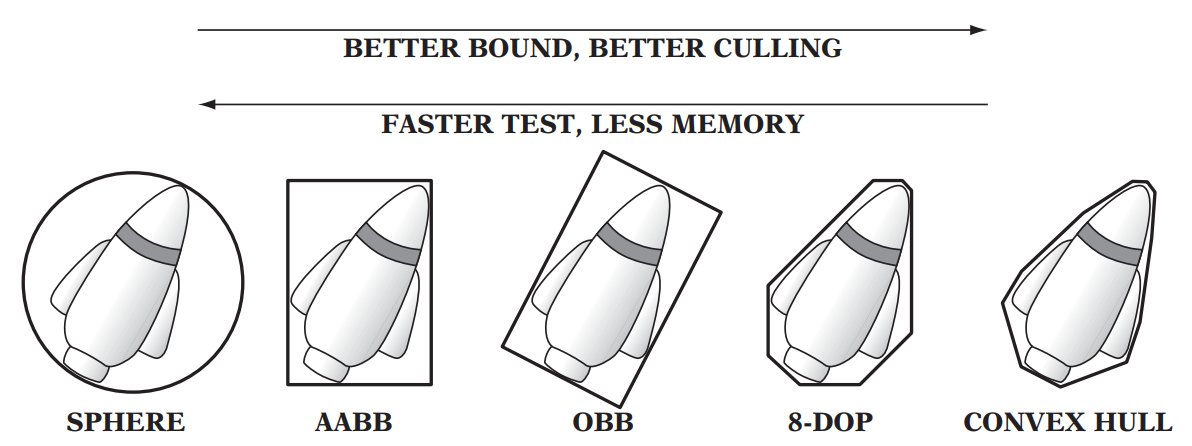
\includegraphics[width=0.75\textwidth]{boundingvolumes}
	\caption{Different types of bounding volumes. \protect\cite{ericson2004real}}
\end{figure}
Ideally, we would like our bounding volume to be as tightly enclosed as possible but also easier to check for an intersection with a ray. A tight bounding volume would help us to have the least amount of overlaps with other bounding volumes in our scene while a fast intersection test would help reducing time complexity. One popular bounding volume type is \textbf{AABB} or \textbf{Axis-Aligned Bounding Box} (also shown in figure 15). This is due to the fact that they are faster to compute (linear run time) and also have a simple intersection test. AABBs are also conventionally preferred over other bounding volumes when building bounding volume hierarchies and so we will use the same in our implementation.
\\~\\
\noindent
Since, now we have an intuition about what a bounding volume means, we can discuss what a hierarchy of such volume(s) would mean. The idea is to partition complex objects into a hierarchy of nodes or sets which contains only a smaller portion of the whole complex object. Looking at figure 15 (AABB) again, we can notice that we are using just one bounding volume to enclose the whole rocket model but we can surely divide the model into two parts. This can be done horizontally so that the nose of the rocket is in a separate AABB and the bottom portion with the wings and the body in a separate AABB. This can also be done vertically, separating the body and the wings in two different AABBs. Figure 16 visualizes the concept using a simpler scene. 
\\~\\
\noindent
In the figure we can see that the whole scene itself is first enclosed into one big bounding volume and then that bounding volume encloses two other bounding volumes. These two bounding volumes contain the primitives themselves but those primitives are also enclosed using a simpler bounding volume (AABB).
\begin{figure}[H]
	\centering
	\captionsetup{justification=centering,margin=2cm}
	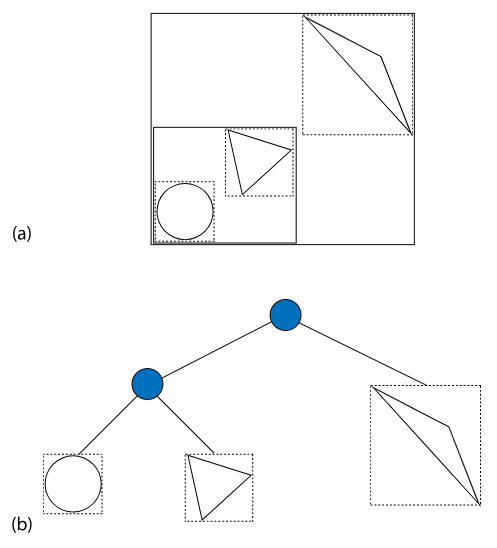
\includegraphics[width=0.35\textwidth]{bvh_pbr}
	\caption{A hierarchy of bounding volumes of a scene consisting of 3 primitives. \protect\cite{pharr2016physically}}
\end{figure}
The idea here is to partition complex objects into a hierarchy of simpler objects that are easier to test. If we send a ray into the scene shown in figure 16, our first test would be with the scene AABB itself (a), and if our ray does intersect with the scene AABB or the root node, we can then move further and test similarly with the two AABBs in the left and right node.  Now there's a chance that our ray hits the left node again where we would test the same ray again but this time only with the primitives' AABBs in the left node. And if our ray does not hit the right node, then that would mean that we also do not intersect with any of the primitives in the right node or for more complex scenes, any of the further nodes in the right node. This results in a much more efficient way to test if we have an intersection with complex models in our scene. This way of dividing objects is known as \textbf{object subdivision}.

\subsection{Implementation}
We do have an idea of how to build the hierarchy or tree of primitives in our scene but there are still some important questions to answer. One of the most important part in a BVH is the \textbf{splitting criteria}. As we go through all the primitives in our scene, we need a criteria that decides how to partition our primitives in the left and right node. This is important because a bad criteria can result in a bad tree where our primitives in both left and right node could overlap. This would result in more ray-primitive intersection tests when the tree is traversed and thereby resulting in a bad implementation of BVH. We will discuss 2 different splitting criterias in this report starting with the most trivial one.
\subsubsection{Splitting Criterias}
\begin{enumerate}
\item \textbf{Randomly sorting axis:}
One way to split the primitives is to sort them by picking a random axis. Once the primitives are sorted, the first half of the primitives can be placed into the left node while the second half can be placed in the right node. This ofcourse does not take into account many of the information in our scene that could be helpful but is still quite fast than not using the acceleration structure at all. Figure 17 illustrates this method for a simple scene.
\begin{figure}[H]
	\centering
	\captionsetup{justification=centering,margin=2cm}
	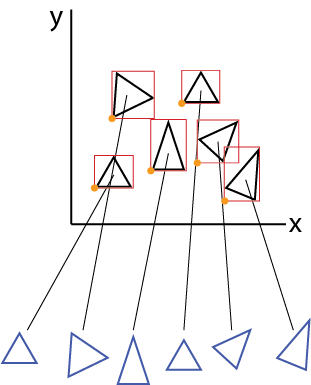
\includegraphics[width=0.3\textwidth]{sorting_bvh}
	\caption{Sorting primitves in a scene based on x-axis.}
\end{figure}
One important rule here is to not use the same axis for sorting all the nodes in our tree as that would result in a tree biased towards a particular axis. Think of a scene where the objects are scattered more in the y-axis than the x-axis or z-axis. In that case, sorting primitives in the x-axis would result in a bad tree. One good rule is to randomly pick an axis at every node so that the tree is not biased towards a particular axis. Once we have just 1 or 2 primitives left in our node, we can initialize a leaf node and place the primitive in it.

\item \textbf{Centroid method:}
Another splitting criteria which makes use of some information in our scene in order to split primitives in a node is the centroid method. The method starts with computing the centroid/midpoint of all primitives' AABBs in a node. This is done by first calculating the AABB of a primitive, and then calculating centroid $\boldsymbol{c}$ as:
\begin{equation}
\boldsymbol{c} = (\boldsymbol{primitive_{AABB_{min}}}*0.5)+(\boldsymbol{primitive_{AABB_{max}}}*0.5)
\end{equation}
As we are computing centroids, we can get the minimum and maximum for all the centroids in a node. This minimum and maximum of all centroids is then used to compute an AABB which represents the AABB based on centroids of all the primitives in this node. Once we have this AABB, we then compute the diagonal $\boldsymbol{d}$ of this AABB as:
\begin{equation}
\boldsymbol{d} = \boldsymbol{AABB_{max}} - \boldsymbol{AABB_{min}}
\end{equation}
\begin{figure}[H]
	\centering
	\captionsetup{justification=centering,margin=2cm}
	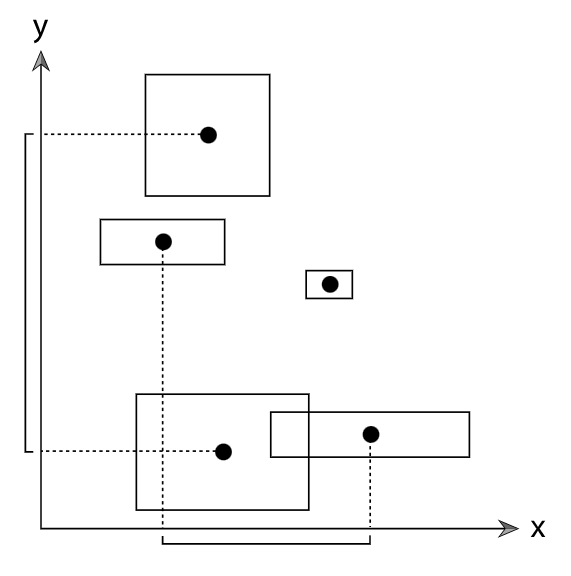
\includegraphics[width=0.3\textwidth]{centroid_bvh}
	\caption{Splitting primitves in a scene based on centroids of their bounding volumes. Note that here, splitting in y-axis is the best way to split primitives.\protect\cite{pharr2016physically}}
\end{figure}
This diagonal $\boldsymbol{d}$ can then be used to find the maximum extent in a given axis. What this means is that, we check the $x$, $y$ and $z$ value of this diagonal $\boldsymbol{d}$ and the one which is the highest among the three is the axis we will use to split our primitives. Intuitively, what we did is chose the axis which results in the least overlap of all AABBs in a given node. 
\\~\\
In the example in Figure 18 above, this axis is $y$ for that specific scene. Remember that previously we were choosing this axis randomly, so this means that with this method, we will surely end up with a better tree as we are using some of the information we have in our scene to select our axis. We still haven't decided the value which would partition our primitives. That part is quite simple. We just need to use the centroid AABB $\boldsymbol{c}$ we calculated previously, and calculate the midpoint of just the splitting axis we computed. So if the best splitting axis was $y$ we compute this split value $s$ as:
\begin{equation}
s=(c_{min_{y}} * 0.5) + (c_{max_{y}} * 0.5) 
\end{equation}
Ofcourse, if the best axis was $x$ or $z$ in another node, we need to use that axis in the above equation. In figure 18 above, this value we just computed is the midpoint of the extent in $y$ so we end up with 2 primitives in the left node and 3 primitives in the right node. There is one slight issue with this approach. If all of the centroid points are at the same position (the centroid bounds have zero volume), we need to stop recursion and introduce a leaf node there. The condition is to check if the centroid AABB $\boldsymbol{c}$'s minimum value at the splitting axis is equal to it's maximum value at the splitting axis. For splitting axis $y$ this condition is:
\begin{equation}
c_{min_{y}} == c_{max_{y}}
\end{equation}
If the condition above is true for any splitting axis, we stop recursion and place first half of the primitives in left node and second half of the primtives in the right node.
\end{enumerate}
\subsubsection{Illustrated example}
The construction of the BVH using centroid split method is illustrated using the same scene as before:
\begin{figure}[H]
	\centering
	\captionsetup{justification=centering}
	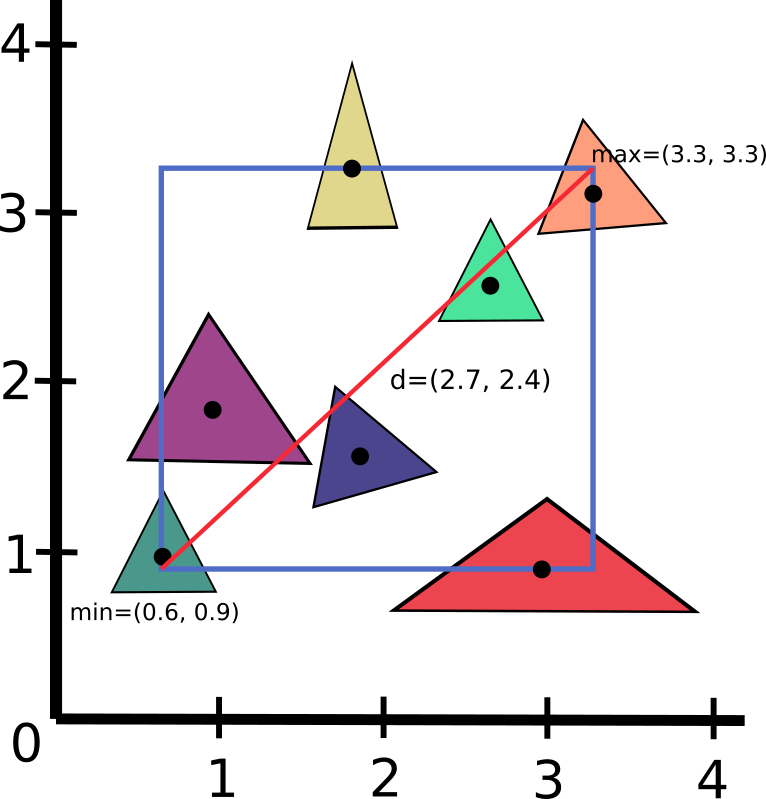
\includegraphics[width=.4\textwidth]{bvh_1}\quad
	\caption{Bounding box of centroids of scene primitives with $\boldsymbol{d}$ calculated.}
\end{figure}
We can see that $\boldsymbol{d}=(2.7, 2.4)$ and we need to split in x-axis for our root node ($2.7 > 2.4$). The split value is then $(0.6*0.5) + (3.3*0.5)=1.95$. And we can partition primitives in the left and right node as:
\begin{figure}[H]
	\centering
	\captionsetup{justification=centering}
	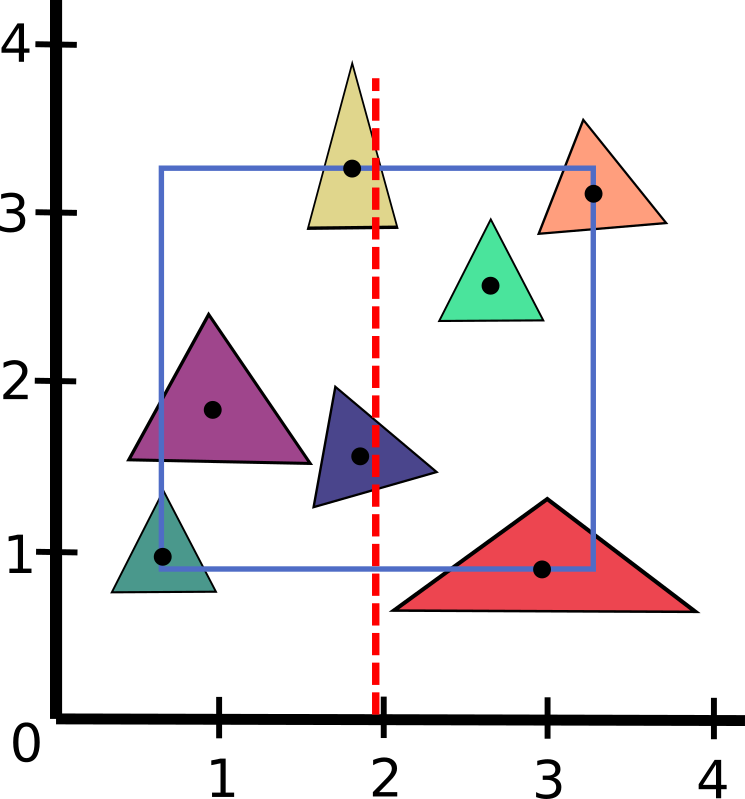
\includegraphics[width=.25\textwidth]{bvh_2}\quad
	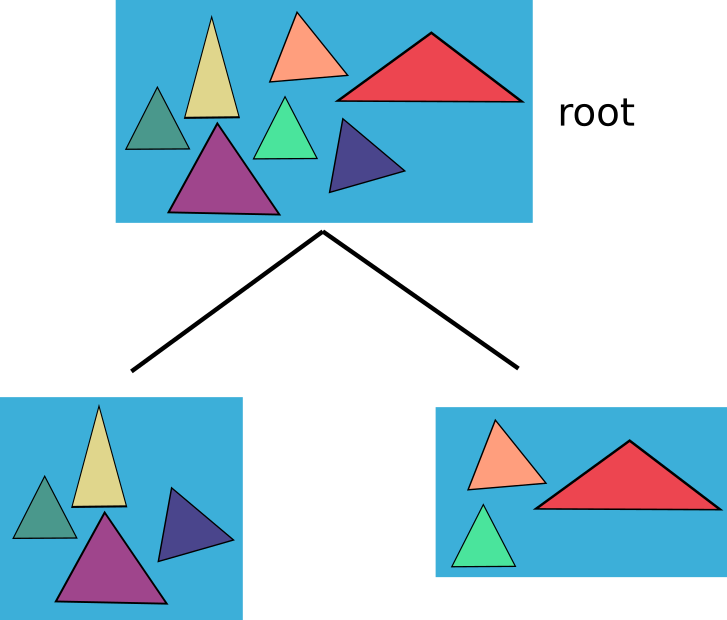
\includegraphics[width=.25\textwidth]{bvh_3}\quad
	\caption{Split point to partition primitives in left and right node (left). Primitives partitioned in left and right node (right).}
\end{figure}
\begin{figure}[H]
	\centering
	\captionsetup{justification=centering}
	\includegraphics[width=.25\textwidth]{bvh_4}\quad
	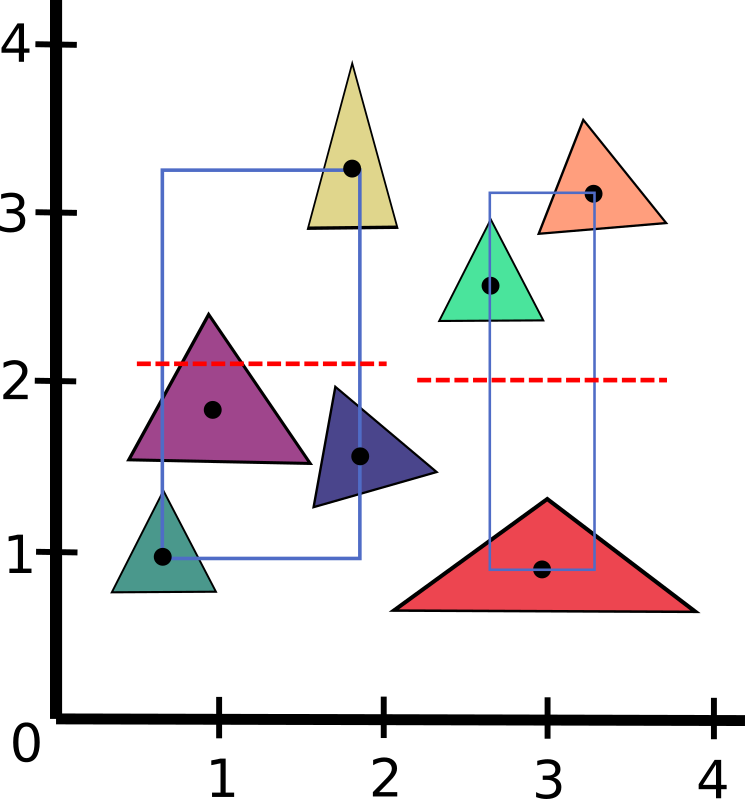
\includegraphics[width=.25\textwidth]{bvh_5}\quad
	\caption{Diagonal $\boldsymbol{d}$ in the left and right nodes (left). Split point in the left and right nodes (right).}
\end{figure}
\noindent
Note that this time, the split was in y-axis because that results in the least number of overlaps ($d_{y} > d_{x}$). Thus the partition continues in the same way until we have only one primitive left, or if the centroid bounds have zero volume.
\begin{figure}[H]
	\centering
	\captionsetup{justification=centering}
	\includegraphics[width=.3\textwidth]{bvh_6}\quad
	\includegraphics[width=.29\textwidth]{bvh_7}\quad
	\caption{Partition in left and right nodes (left). The whole tree (right).}
\end{figure}

\subsubsection{Traversal}
The traversal for a BVH is quite simple. We start with the root node and check if our ray intersects with the AABB of this node. If it doesn't intersect the node, we return from the function but if it does intersect with the node, we then call the function again passing the left and right nodes as parameters. We need a stopping condition for this recursion. We have already discussed one condition i.e we return $false$ if the ray does not intersect this node. One other condition is to check if we have reached a leaf node. This is done by keeping a boolean variable with each node and setting it to $true$ when initializing a leaf node while constructing the tree. Now if we reach a leaf node in our traversal we need to check if the ray intersects with any of the primitives in this leaf node. Unfortunately, since this is the last node in our tree it is necessary to check all primitives in this node to get the closest hit point for our ray. In the accompanied ray tracer, these hit points are saved separately and the closest one is choosen to be shaded. The array for hit points is then cleared and filled again in the next traversal. There is one condition that lets recursion stop early for shadow rays. If a ray is a shadow ray, the first hit found is enough and we can then return from the function. In order to achieve this a boolean is set to $true$ specifically for shadow rays which lets the recursion stop earlier and return from the function.
\subsubsection{Algorithm}
\begin{algorithm}
	\caption{BVH\_traverse}\label{alg:cap}
	\begin{algorithmic}
		\Require $root$, $ray$, $t_{min}$, $t_{max}$, $hit$
		\If{$root$ $\rightarrow$ $AABB$ $\rightarrow$ $intersect(ray, t_{min}, t_{max}) = false$}
			\State $return\;\;false$
		\EndIf
		\If{$root$ $\rightarrow$ $isleaf$}
			\State $hit_{temp} \leftarrow hit$
			\State $bool_{hit} \leftarrow false$
			\State $closest \leftarrow t_{max}$
			\For{$i \gets 0$ to $root$ $\rightarrow$ $N_{primitives}$}                 
			\If{$root$ $\rightarrow$ $primitives[i]$ $\rightarrow$ $hit(ray, t_{min}, closest, hit_{temp})$}
			\If{($ray$ $\rightarrow$ $shadow_{ray}$ $=$ $true$)}
			\State $return$ $true$ 
			\EndIf
			\State $closest \leftarrow hit_{temp}$ $\rightarrow$ $t$
			\State $hit \leftarrow hit_{temp}$
			\State $hits_{save}<vector>$ $\leftarrow$ $hit$
			\State $bool_{hit} \leftarrow true$
			\EndIf
			\EndFor
			\State $return$ $bool_{hit}$
		\EndIf
		
		\State $bool_{hit_{L}}$ $=$ $BVH\_traverse(root$ $\rightarrow$ $left, ray, t_{min}, t_{max}, hit)$
		\State $bool_{hit_{R}}$ $=$ $BVH\_traverse(root$ $\rightarrow$ $right, ray, t_{min}, t_{max}, hit)$
	
		\State $return$ $bool_{hit_{L}}$ $\Or$ $bool_{hit_{R}}$
	\end{algorithmic}
\end{algorithm}
\pagebreak
\section{Analysis}
The data structures implemented in this report were tested on different models. Some obj variants of the scanned models from \emph{The Stanford 3D Scanning Repository} were used. This includes \emph{Stanford Bunny}, \emph{Stanford Lucy}, \emph{Stanford Dragon}, \emph{Stanford Asian Dragon} and \emph{Happy Buddha} \cite{buddha}. The famous \emph{Utah teapot} is also used as well as \emph{Suzanne} \cite{blendermonkey} from Blender and \emph{Spot} from Caltech.
\\~\\
The ray tracer as well as all the methods discussed in the report were implemented in C++. All of the methods also make use of STL. No low level optimizations were made. All results were obtained on a computer with a Quad Core AMD Ryzen 5 PRO 3500U CPU and 16GB of RAM. All images were rendered on a single core. All images use an aspect ratio of $1:1$ and a resolution of $500 \times 500$.  Phong illumination model was used to shade all objects with just one point light in front of the camera. Only 1 ray per pixel was used to render all images. In the tables, BVH\_C is BVH with centroid split method, BVH\_R is BVH with random sorting of axis and C.G is compact grid.
\\
\begin{table}[ht] 
\centering 
{\footnotesize
\begin{tabular}{ P{2.5cm} ||P{2.5cm}  P{2.5cm}  P{2.5cm} P{2.5cm}  }      % centered columns (3 columns) 
\hline\hline                                      %inserts double horizontal lines
& Suzanne  & Spot & Teapot & Bunny \\ [0.5ex] % inserts table heading 
\hline
       & \Includegraphics[height=1in]{figures/suzanne}& \Includegraphics[height=1in]{figures/spot} & \Includegraphics[height=1in]{figures/teapot} & \Includegraphics[height=1in]{figures/bunny} \\
\hline
    \end{tabular}
}
\end{table}
\vspace{-2em}
\begin{table}[ht] 
\centering 
{\footnotesize
\begin{tabular}{ P{2.5cm}||P{2.5cm}P{2.5cm} P{2.5cm} P{2.5cm}  }      % centered columns (3 columns) 
\hline
\\
\#tri's & 968  & 5, 856 & 15, 704 & 69, 451 \\ [0.5ex] % inserts table heading 
\\
\hline \hline
\\
BVH\_C build(s)& 0.014 s& 0.091 s & 0.26 s & 1.3 s \\
\\
BVH\_R build(s)& 0.03 s& 0.3 s & 0.84 s & 5.1 s \\
\\
C.G build(s)& 0.0013 s& 0.005 s & 0.015 s & 0.07 s \\
\\
\hline \hline
\\
BVH\_C render(s)& 1.1 s& 1.34 s & 1.36 s & 1.5 s \\
\\
BVH\_R render(s)& 2.8 s& 23.2 s & 5.7 s & 25.5 s \\
\\
C.G render(s)& 1.17 s& 1.5 s & 1.4 s & 2.4 s \\
\\
\hline \hline
\\
BVH\_C avg \# isect tests / isect ray& 56.004& 64.107& 98.9& 76.1 \\
\\
BVH\_R avg \# isect tests / isect ray& 185& 488& 703& 2100 \\
\\
C.G avg \# isect tests / isect ray& 34.31& 41.088& 41.35& 71.6 \\
\\
\hline \hline
    \end{tabular}
}
\end{table}

\pagebreak

\begin{table}[ht] 
\centering 
{\footnotesize
\begin{tabular}{ P{2.5cm} ||P{2.5cm}  P{2.5cm}  P{2.5cm} P{2.5cm}  }      % centered columns (3 columns) 
\hline\hline                                      %inserts double horizontal lines
& Lucy  & Asian Dragon & Dragon & Happy Buddha \\ [0.5ex] % inserts table heading 
\hline
        & \Includegraphics[height=1in]{figures/lucy}& \Includegraphics[height=1in]{figures/xyz_dragon} & \Includegraphics[height=1in]{figures/dragon} & \Includegraphics[height=1in]{figures/buddha} \\
\hline  
    \end{tabular}
}
\end{table}
\vspace{-2em}
\begin{table}[ht] 
\centering 
{\footnotesize
\begin{tabular}{ P{2.5cm}||P{2.5cm}P{2.5cm}  P{2.5cm} P{2.5cm}  }      % centered columns (3 columns) 
\hline
\\
\#tri's & 99, 970  & 249, 999 & 871, 306 & 1, 087, 474 \\ [0.5ex] % inserts table heading 
\\
\hline \hline
\\
BVH\_C build(s)& 1.97 s& 5.4 s & 20.8 s & 26.17 s \\
\\
BVH\_R build(s)& 8.1 s& 22.5 s & N/A & N/A \\
\\
C.G build(s)& 0.1 s& 0.22 s & 0.8 s & 0.98 s \\
\\
\hline \hline
\\
BVH\_C render(s)& 1.18 s& 1.68 s & 2.62 s & 1.91 s \\
\\
BVH\_R render(s)& 31.4 s& 24.3 s & N/A & N/A \\
\\
C.G render(s)& 2.1 s& 3.5 s & 5.7 s & 4.28 s \\
\\
\hline \hline
\\
BVH\_C avg \# isect tests / isect ray& 85.965& 100.97& 95.64& 98.06 \\
\\
BVH\_R avg \# isect tests / isect ray& 2728.2& 3264.3& N/A& N/A \\
\\
C.G avg \# isect tests / isect ray& 59.12& 115.89& 155.68& 116.7 \\
\\
\hline \hline
    \end{tabular}
}
\end{table}

For all of the scenes we record the time it takes to construct the data structure and the time it takes to render the image. Another metric which is quite helpful is to compute the average number of intersection tests per intersecting ray. So, for every ray that intersects with the scene bounding box, we compute the number of intersection tests, sum them all together, and then take the average of it by dividing it by the number of intersecting rays. It can be seen that both compact grids as well as the BVH centroid split method perform really well on a variety of 3D models with different number of triangles. 

\subsection{Construction time analysis}
\subsubsection{Why compact grid is fast to construct?}
Overall, it can be seen that compact grid takes less time to build as compared to the binary tree in BVH centroid split method. This is because compact grid is constructed by first going through all primitives in the scene, check which cells they overlap to get the linearized $C$ array, so it is a loop over all primitives in the scene. Then the linearized $C$ array is corrected by going through the same array itself. This array has approximately the size of the density $\rho$ times the primitives in our scene. Next, we allocate the object list $L$ by using the value in the last index of $C$. Once we have both these arrays, we then get the corrected $L$ and $C$ array by reversely iterating through the primitives once again, getting the cell they overlap and then getting the final $L$ and $C$ array. We can ofcourse, save much of the information previously when we go through the primitives array the first time, but it would require a lot of additional memory because one triangle can be in more than one cell so this array which would store this information would be quite large. Overall, most of the time is spent checking for triangles that overlap with the voxels in our scene but since we only have to go through them two times, it is quite fast.

\subsubsection{Why current BVH implementation is slow to construct?}
Comparing this with the BVH centroid split method, we start with the scene bounding box which is the root node of our tree. This contains all of the primitives in our scene, so we go through them one by one, get their bounding boxes, get the centroid of those bounding boxes, and then compute the union of all those centroids to get a resultant bounding box. This resultant bounding box is then used to get the best split for the primitives in the current node and then we partition them into left and right nodes. Note that for both left and right nodes, we again want the correct bounding box that encloses the primitives in those nodes, so we again want a union of all bounding boxes of primitives in each of those nodes. This process is repeated for the left and right nodes again until we reach our base condition. So, most of the time is spent computing this resultant bounding box, which requires us to loop through all primitives in a node. This makes this BVH slow to construct. One important thing to mention here is that the better the split criteria, the better the quality of our tree, and the less the depth of our tree. So as a result, if we use a better criteria, we would be able to partition the primitives in a much better way, and this would result in a tree with less overlapping primitives in both left and right nodes of our tree. This can help in cutting down the time it takes to construct the tree in some scenarios (depending on the complexity of the splitting criteria) but would always help in cutting down the render time.
\\~\\
The BVH random split method performs poorly compared to other structures. This is quite obvious since we choose the split axis randomly without using any valuable information our scene can give to us. We sort the primitives and then place the first half in left node and the second half in the right node. Choosing the split axis randomly also results in random trees. In some cases, the tree is satisfactory while in other cases the tree can be much worse, increasing both the time complexity as well as the space complexity for tree construction. During the analysis, each scene was rendered 4 times and an average was taken for all values. Resulting in a bad tree also increases the render time since then there might be a case that many of the primitives end up in both left and right nodes of our tree with wasted repeated intersection tests.

\subsection{Render time analysis}
Let's discuss the render time now. This is the amount of time it takes to render our image given that we have already built our data structure. It can be seen that both compact grids and BVH centroid split method perform quite nicely and render the image in similar times. One deviation to notice is the fact that the render time for compact grids is increasing slightly as the number of triangles in our scene increase. This is not true for BVH. The centroid split method for BVH renders the Happy Buddha scene in about 1.91 seconds, which is almost the same amount of time it takes for all other scenes. The compact grid however, while still very fast for less complex scenes, starts to take more time to render the image for more complex scenes. The Happy Buddha scene takes about 4.28 seconds, while the Suzanne scene takes just about 1.17 seconds to render for the compact grid.
\\~\\
Let's discuss the metric we computed which is the average number of intersection tests for each intersecting ray. It is interesting to note that this metric has a direct relation to the render time. If the value is lower, this would mean that the image would also take less time to render. Higher values can result in an increased render time. So for example, the dragon scene has the value $155.68$ for compact grids and the time it takes to render the scene with compact grids is about 5.7 seconds. The same scene has a value of $95.64$ for BVH, and it takes about 2.62 seconds to render the image using BVH. This metric can also be used to come up with a better density $\rho$ value for a specific scene when using compact grids. This value, as mentioned previously is used in equation (2) to get the desired grid resolution. Let's discuss this further for a more complex scene.

\subsection{Further analysis}
\begin{table}[ht] 
\centering 
{\footnotesize
\begin{tabular}{ P{2.5cm} ||P{6cm} || P{6cm}  }      % centered columns (3 columns) 
\hline\hline                                      %inserts double horizontal lines
& Scene 1 & Scene 2\\ [0.5ex] % inserts table heading 
\hline
        & \Includegraphics[height=1.35in]{figures/custom_scene}& \Includegraphics[height=1.35in]{figures/benchmark_scene} \\
\hline  
    \end{tabular}
}
\end{table}
\vspace{-2em}
\begin{table}[ht] 
\centering 
{\footnotesize
\begin{tabular}{ P{2.5cm}||P{6cm} P{6cm}  }      % centered columns (3 columns) 
\hline
\\
\centering \#tri's & 3, 362, 633 $\approx$ 3.36M & 1, 401, 384 $\approx$ 1.4M  \\ [0.5ex] % inserts table heading 
\\
\hline \hline
\\
BVH\_C build(s)& 95.91 s & 36.12 s \\
\\
C.G build(s)& $(\rho=4)$\:3.7 s, $(\rho=10)$\:4.6 s, $(\rho=15)$\:5.72 s& $(\rho=8)$\:1.48 s, $(\rho=15)$\:1.8 s, $(\rho=30)$\:2.75 s  \\
\\
\hline \hline
\\
BVH\_C render(s)& 100.15 s & 1906 s \\
\\
C.G render(s)&  $(\rho=4)$\:206.5 s, $(\rho=10)$\:150.5 s, $(\rho=15)$\:133.94 s& $(\rho=8)$\:6707 s, $(\rho=15)$\:4621 s, $(\rho=30)$\:4365 s  \\
\\
\hline \hline
\\
BVH\_C avg \# isect tests / isect ray& 320.96 & 79.69\\
\\
C.G avg\# isect tests / isect ray& $(\rho=4)$\:551.996, $(\rho=10)$\:364.94, $(\rho=15)$\:314.26& $(\rho=8)$\:260.717, $(\rho=15)$\:193.07, $(\rho=30)$\:143.08 \\
\\
\hline \hline
    \end{tabular}
}
\end{table}

\subsubsection{Scene 1}
This scene uses an aspect ratio of $16:9$ with a resolution of $1000 \times 562$. 3 rays per pixel were used to render this scene. 2 point lights, one in front of the camera with an intensity value of $30$ and the other above the scene with a high intensity value of $60$ were used. Special thanks to \cite{grass} for the grass 3D model. The scene uses random scaling for the grass so that it properly represents a natural scene. This affects the render time as well as build time slightly for different runs but not so much.
\\~\\
It is interesting to note that BVH outperforms compact grid in this scene at first. The build time is about $95$ seconds and the render time is about $100$ seconds with a total of about $195$ seconds for time to image. Compact grids while still take less time to construct ($3.7$ seconds), the time taken to render the image is about $206$ seconds with a total of about $209.7$ seconds. Note that the average number of intersection tests per intersecting ray for compact grids is quite high ($551.996$) compared to BVH ($320.96$). Now we tried to increase the value $\rho$ to get different resolution grids for compact grid and noticed that they start to get better results for increased density. 
\\~\\
For a value of $\rho=10$ the average number of intersection tests per intersecting ray went down to $364.94$ which had a significant impact on render time as well. This time we were able to render the same image in about $155$ seconds, which is about $55$ seconds faster than before. Now increasing the $\rho$ value further to $15$ gives us a value of $314.26$, rendering the image in about $134$ seconds. The total time to image is now about $140$ seconds. Note that we have already outperformed BVH for this scene which had total time to image of about $195$ seconds. The metric we computed can therefore be used to arrive at a better $\rho$ value for specific scenes when using compact grids. Let us analyze one more scene, this time using area lights and having different objects of varied number of triangles scattered throughout the scene.
\subsubsection{Scene 2}
This scene uses an aspect ratio of $16:9$ with a resolution of $1000 \times 562$. 5 rays per pixel were used to render this scene. This time five area lights were used instead of point lights. All of them are basically point lights in a grid of $3 \times 3$ so a total of $45$ point lights. The intensity value for a point is then averaged by total number of point lights in each area light to compute shading. All of the lights are mostly around the center of the scene. As you can notice, the scene has different objects with varied amount of triangles; some of them are highly dense objects while others contain less number of triangles.
\\~\\
Compact grids perform very poorly in this scene. As obvious from the table, the construction time was quite low (about $1.5$ seconds) but rendering this scene took about $6707$ seconds or about $1$ hour $50$ minutes. Increasing the density $\rho$ value helps a bit but even increasing it to a value of $30$ takes it down to $4365$ seconds or about $1$ hour $12$ minutes. The reason behind this significant impact even though the scene contains almost half of the number of triangles in scene 1 is because this scene has a \textbf{non uniform primitive distribution}. This causes uniform grids to suffer from a problem known as \textbf{teapot in a stadium} \cite{utahteapot} problem. What this means is that, if all objects in the scene have approximately the same size, then uniform grids have generally good results, but if there are objects which contain a small number of primitives and some objects that contain a very high density of primitives, then many of the primitives end up in many cells of the grid which results in greater number of intersection tests in some cells resulting in poor performance. An improvement over the regular compact grids was made in the paper \textbf{Two-Level Grids for Ray Tracing on GPUs} \cite{kalojanov2011two} which constructs two levels grids depending on the density of primitives in a particular region. When a region of high density is found, another grid with an increased density is introduced in the region. This helps in handling the problem of non uniform primitive distributions more robustly.
\\~\\
BVH however, do not suffer from this problem since it divides objects (object subdivision) instead of space (space subdivision). This is the reason why BVH was able to render the same scene in about $1906$ seconds or about 31 minutes. But this also does not mean that BVH will outperform uniform grid in every scenario. 
\\~\\
In our previous scenes which contained single models with approximately uniformly distributed primitives, the compact grid implementation outperformed BVH in the total time to image (construction and render time). The Happy Buddha scene for instance, takes about 27 seconds for BVH while it takes just about 6 seconds for compact grid. This tells us that BVH is mostly ideal for sparse scenes \cite{boulos2005notes} where we can group objects into two separate clusters that may be separated by large portions of space. Another important aspect is the memory consumption. Compact grids allocates memory according to the resolution of the grid (equation (2)) while the current BVH implementation keeps pointers to primitives in each node making compact grids, a better choice for representing complex scenes efficiently.

\section{Conclusion}
In this report, we started our discussion with the importance of acceleration structures in ray tracing. We went through a spatial subdivision technique known as uniform grid and discussed an implementation to compactly represent a uniform grid using two static arrays. We then went through an algorithm to efficiently traverse this grid. Afterwards, we discussed an object subdivision technique known as bounding volume hierarchies. We then went through an implementation of BVH which can be used to build an efficient hierarchy. Afterwards, we analysed these two structures and noticed that they perform differently in different scenes. The BVH performed better in scenes where the objects are dense but also separated by large portions of space. While the compact grid was the better choice in scenes where the objects are dense but also uniformly distributed. This tells us that it is often difficult to find a structure that works best in all scenarios and it is a matter of testing different structures and choosing the one that works best in our case.
\\~\\
\noindent
The author thanks his supervisor \textbf{Prof.
	Dr.-Ing. Matthias Teschner} once again for the guidance throughout this project.
 
\bibliographystyle{apacite}
\bibliography{References}
\end{document}